% !TeX root = ../main.tex
\section{Wichtigkeit von Knoten \& Knotengruppen}
\label{sec:zentralitaet}

Wir messen die Zentralität im Arbeitsnetz mit 13\,156 Athleten und
357\,219 Kanten. Degree und Weighted Degree berechnen wir für alle Athleten.
Closeness, Betweenness und Eigenvector setzen einen zusammenhängenden Graphen
voraus und beziehen sich deshalb auf die Giant Component mit 12\,709
Athleten. Die Kantengewichte verwenden wir nur beim Weighted Degree, der die
gemeinsamen Tage mit allen Nachbarn summiert. Für Distanzen eignen sie sich
nicht, da ein hohes Gewicht eine engere Verbindung bedeutet und keine
längere Strecke. Die Closeness berechnen wir als normierte Summe der
inversen Distanzen
\[
  C_H(v)=\frac{1}{n-1}\sum_{u\ne v}\frac{1}{d(u,v)}.
\]
Prestige-Masse entfallen, da unser Netz ungerichtet ist.

\subsection{Zentrale Athleten}
Abbildung~\ref{fig:zentralitaet_athleten} zeigt die fünf höchsten Werte je
Mass. Den höchsten Degree hat Katinka Hosszú mit 543 Nachbarn, sie erreicht
auch die höchste Closeness. Ein hoher Degree bedeutet bei uns aber nicht
viele Wettkämpfe. Hosszú ist an 41 Veranstaltungstagen erfasst, Sheng-Yo
Ting mit 498 Nachbarn sogar nur an 12. Der Median aller Athleten liegt bei
16 Tagen. Viele Nachbarn entstehen also durch wenige, aber sehr grosse
internationale Veranstaltungen.

Die Eigenvector-Zentralität ist hoch, wenn die Nachbarn selbst zentral sind.
Alle zehn höchsten Werte liegen im innersten k-Core aus
Kapitel~\ref{sec:communities}, also bei Athleten der Weltmeisterschaft 2009
in Rom. Von den ersten hundert sind es 76\,\%. Darunter sind auffällig viele
Athleten kleiner Nationen wie Simbabwe, Macau, Namibia oder der Cayman
Islands. Für sie ist eine Weltmeisterschaft oft der Ort ihrer Bestleistung,
wodurch sie im dichtesten Teil des Netzes liegen.

\begin{figure}[H]
  \centering
  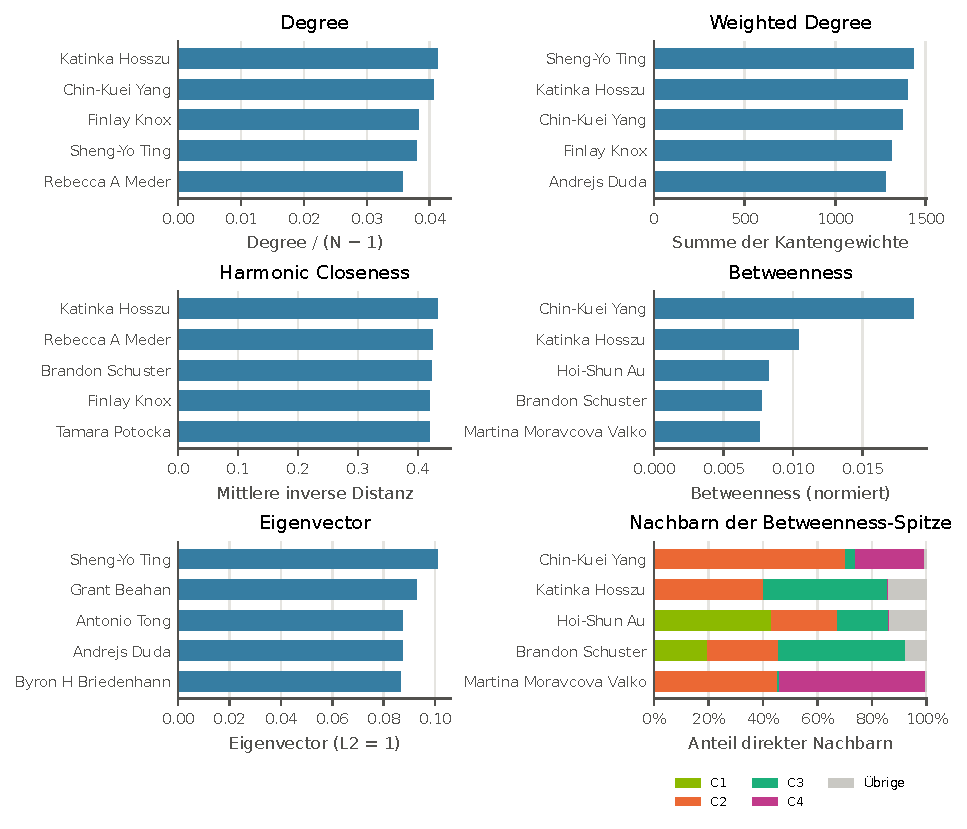
\includegraphics[width=\textwidth]{06_zentralitaet_athleten.pdf}
  \caption{Die fünf höchsten Werte je Mass. Degree und Weighted Degree für
  alle Athleten, die übrigen Masse für die Giant Component. Unten rechts
  die direkten Nachbarn der fünf Athleten mit der höchsten Betweenness nach
  Community. Eigene Auswertung.}
  \label{fig:zentralitaet_athleten}
\end{figure}

Die Betweenness misst, wie oft ein Athlet auf kürzesten Wegen zwischen
anderen liegt. Die höchsten Werte haben Chin-Kuei Yang (0,0187), Hosszú
(0,0104) und Hoi-Shun Au (0,0083). Au hat nur 156 Nachbarn und liegt beim
Degree auf Rang 690. Alle zehn Athleten mit der höchsten Betweenness haben
Nachbarn in mindestens drei der vier Generationen aus
Kapitel~\ref{sec:communities}. Yang verbindet vor allem C2 (375 Nachbarn)
mit der älteren C4 (135), Martina Moravcová Valko ebenso C4 (94) mit C2
(80). Jan Sefl verbindet dagegen die fast vollständig tschechische
Community C32 mit den internationalen Generationen. Von seinen 219 Nachbarn
liegen 132 in C1 bis C3. Hohe Betweenness kennzeichnet somit Athleten an
den Übergängen zwischen Generationen oder zwischen nationaler und
internationaler Ebene.

Tabelle~\ref{tab:zentralitaet_beispiele} ordnet vier bekannte Athleten ein.
Michael Phelps liegt bei keinem Mass unter den ersten 100 und bei der
Betweenness nur auf Rang 1\,376. Von seinen 168 Nachbarn liegen 155 in C2,
eine Brücke zwischen Generationen ist er im Netz also nicht. László Cseh
liegt dagegen bei Betweenness (Rang 23) und Closeness (28) deutlich höher
als beim Degree (131). Moravcová Valko erreicht bei der Betweenness sogar
Rang 5, beim Degree nur Rang 517.

\begin{table}[H]
  \centering
  \caption{Vier ausgewählte Athleten. Werte und in Klammern der Rang, gleiche
  Werte erhalten denselben Rang. C: Community aus Kapitel~\ref{sec:communities}.
  Eigene Auswertung.}
  \label{tab:zentralitaet_beispiele}
  \small
  \setlength{\tabcolsep}{2.5pt}
  \begin{tabular}{@{}lcrrrrr@{}}
    \toprule
    Athlet & C & Degree & Gewichtet & Closeness & Betweenness & Eigenvector \\
    \midrule
    Katinka Hosszú & 3 & 543 (1) & 1\,398 (2) & 0,4332 (1) & 0,01040 (2) & 0,0727 (26) \\
    Michael Phelps & 2 & 168 (583) & 383 (809) & 0,3633 (855) & 0,00045 (1\,376) & 0,0295 (291) \\
    László Cseh & 2 & 279 (131) & 656 (154) & 0,4041 (28) & 0,00537 (23) & 0,0451 (152) \\
    Martina Moravcová Valko & 4 & 176 (517) & 379 (832) & 0,3553 (1\,243) & 0,00762 (5) & 0,0250 (357) \\
    \bottomrule
  \end{tabular}
\end{table}

Die Masse hängen zusammen, sind aber nicht austauschbar. Die Rangkorrelation
nach Spearman reicht von 0,96 zwischen Degree und Weighted Degree bis 0,47
zwischen Weighted Degree und Eigenvector. Alle Werte beschreiben gemeinsame
Veranstaltungstage gespeicherter Bestleistungen. Hohe Zentralität zeigt
deshalb, an welchen Veranstaltungen ein Athlet seine Bestleistungen
erzielte, und keine persönlichen Kontakte.

\subsection{Leistung und Zentralität}
Sind stärkere Schwimmer zentraler? Als Leistung verwenden wir die maximalen
FINA-Punkte eines Athleten. Für 12\,708 der 12\,709 Athleten der Giant
Component liegt ein Punktewert vor. Wir prüfen den Zusammenhang mit einem
monadischen Permutationstest. Die Nullhypothese lautet, dass Punkte und
Zentralität nicht zusammenhängen. Dazu werden die Punkte 9\,999-mal
zufällig auf die Athleten verteilt, Netzwerk und Zentralitäten bleiben
unverändert. Teststatistik und Effektgrösse ist die Rangkorrelation $\rho$
nach Spearman, das Signifikanzniveau beträgt $\alpha = 0{,}05$.

Alle fünf Zusammenhänge sind positiv
(Abbildung~\ref{fig:zentralitaet_leistung}). Am stärksten sind sie bei der
Closeness ($\rho = 0{,}36$) und der Betweenness (0,33), es folgen
Eigenvector (0,29), Degree (0,23) und Weighted Degree (0,17). Keine
Permutation erreicht einen der beobachteten Werte ($p = 0{,}0001$, nach
Holm-Korrektur für die fünf Tests $p = 0{,}0005$). Stärkere Schwimmer liegen
also näher am Zentrum des Netzes und häufiger auf kürzesten Wegen. Die
Effekte sind aber schwach bis mässig.

\begin{figure}[H]
  \centering
  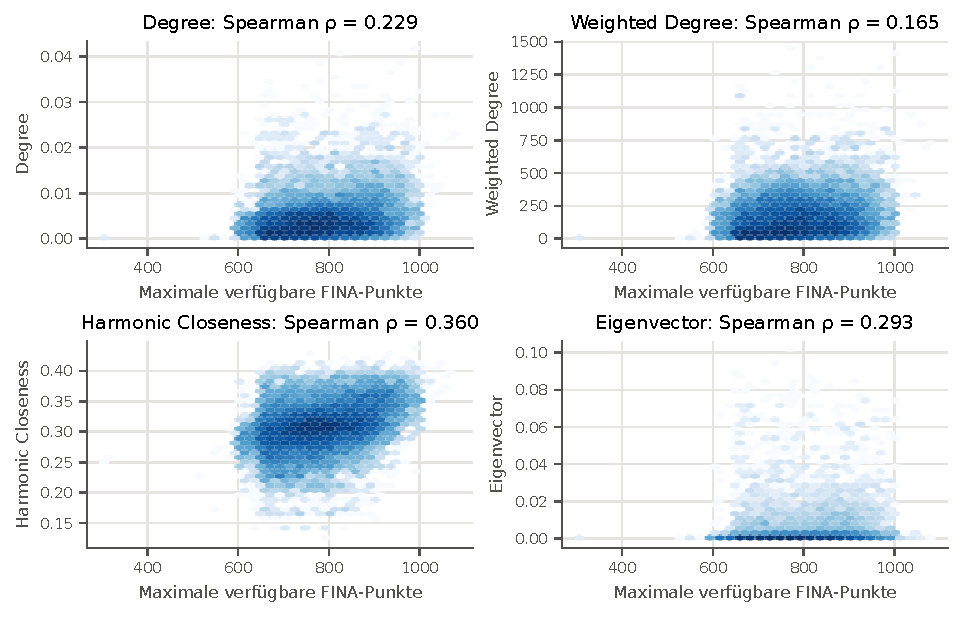
\includegraphics[width=\textwidth]{06_zentralitaet_leistung.pdf}
  \caption{Maximale FINA-Punkte und Zentralität für 12\,708 Athleten der
  Giant Component. Dunklere Felder enthalten mehr Athleten (logarithmische
  Farbskala). Betweenness und Eigenvector mit logarithmischer y-Achse.
  Eigene Auswertung.}
  \label{fig:zentralitaet_leistung}
\end{figure}

Ein Teil des Zusammenhangs kann am Datenumfang liegen. Je Athlet sind 2 bis
100 Bestleistungen gespeichert, im Median 20. Ihre Zahl korreliert sowohl
mit den maximalen Punkten ($\rho = 0{,}27$) als auch mit dem Weighted Degree
(0,49). Der Test belegt deshalb keinen kausalen Einfluss der Leistung.

\subsection{Nationalteams und Generationen}
Für Gruppen von Athleten verwenden wir Degree und Closeness auf
Gruppenebene. Mit $d(v,S)$ als Distanz zum nächsten Mitglied der Gruppe $S$
und $N = 13\,156$ gilt
\[
  C_D(S)=\frac{|\{v\notin S:d(v,S)=1\}|}{N-|S|},\qquad
  C_H(S)=\frac{1}{N-|S|}\sum_{v\notin S}\frac{1}{d(v,S)}.
\]
Der Group Degree ist also der Anteil der Aussenstehenden mit direkter
Verbindung zur Gruppe, die Group Closeness der Mittelwert ihrer inversen
Distanzen. Die Group Betweenness lassen wir weg, da sie für ein Netz dieser
Grösse zu aufwendig ist. Als Gruppen dienen die 22 Nationen mit mindestens
200 Athleten aus Kapitel~\ref{sec:reduktion} und die Generationen C1 bis C4
aus Kapitel~\ref{sec:communities}.

Die USA erreichen mit 206 Athleten 2\,905 Aussenstehende direkt
(Group Degree 0,224) und haben auch die höchste Group Closeness (0,581).
Japan folgt mit 0,217, die Türkei liegt bei beiden Massen am tiefsten
(0,108 und 0,513). Der Group Degree hängt stark mit dem nationalen Anteil
aus Kapitel~\ref{sec:reduktion} zusammen (Spearman $-0{,}82$). Je mehr Tage
die Athleten einer Nation mit Landsleuten teilen, desto weniger
Aussenstehende erreicht das Team.

\begin{figure}[H]
  \centering
  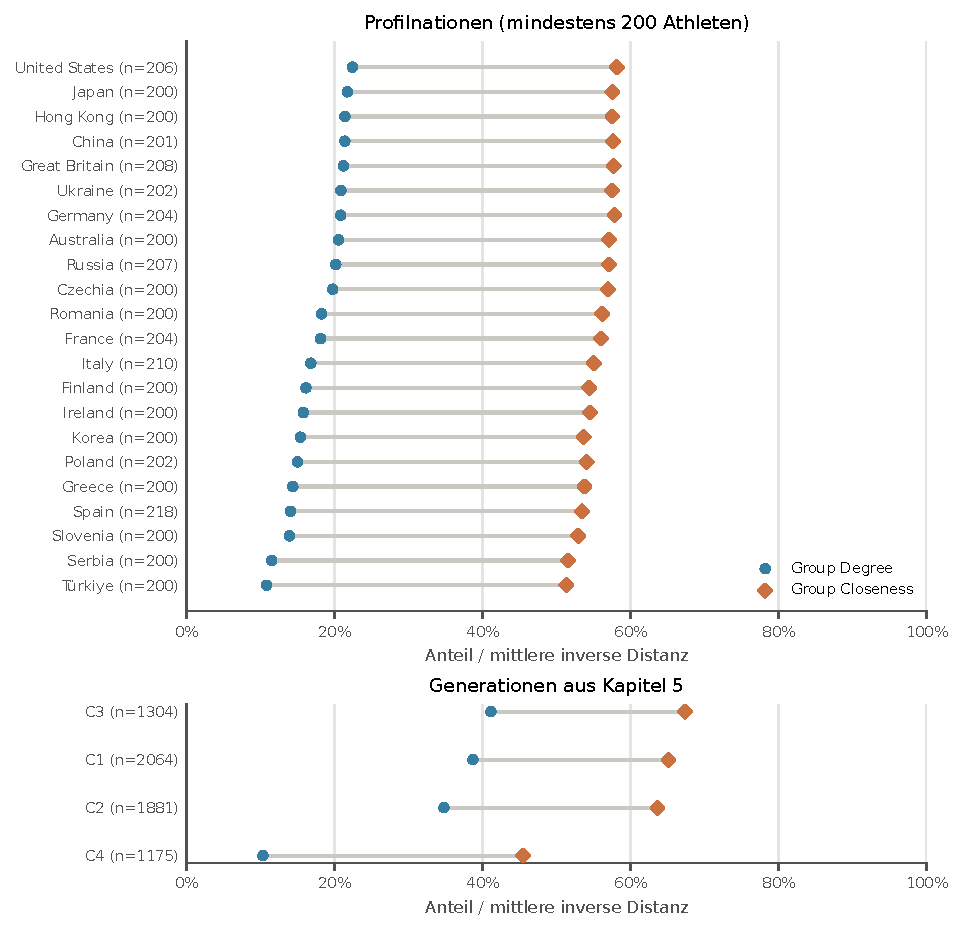
\includegraphics[width=0.88\textwidth]{06_zentralitaet_gruppen.pdf}
  \caption{Group Degree (blau) und Group Closeness (orange) der Nationen mit
  mindestens 200 Athleten und der Generationen C1 bis C4. In Klammern die
  Gruppengrösse. Eigene Auswertung.}
  \label{fig:zentralitaet_gruppen}
\end{figure}

Bei den Generationen ist C3 am zentralsten. Sie erreicht mit 1\,304
Athleten 4\,876 Aussenstehende direkt (0,411) und liegt damit vor der
grösseren C1 (0,387) und C2 (0,348). C3 liegt zeitlich und im Layout von
Abbildung~\ref{fig:communities} zwischen C2 und C1. Die älteste Generation
C4 erreicht dagegen nur 1\,240 Aussenstehende (0,103). Ihre Bestleistungen
stammen vermutlich zu selten von denselben Veranstaltungen wie jene späterer
Athleten. Da die Generationen deutlich grösser sind als die Nationalteams,
vergleichen wir die Werte nur innerhalb der beiden Gruppenarten.
